\documentclass[twoside]{report}
\usepackage[utf8]{inputenc}
%\usepackage[english]{babel}
\usepackage{amsthm}
\usepackage{tkz-fct} 
\usepackage{thmtools}
\usepackage[margin=1in]{geometry}
\usepackage{amsmath,amssymb}
\usepackage{multicol}
\usepackage{graphicx}
\usepackage{tikz}
\usepackage{listings}
\usetikzlibrary{positioning} 
\usetikzlibrary{calc,patterns,angles,quotes}
\usetikzlibrary{calc,arrows, arrows.meta}
\tikzset{
  arrow/.pic={\path[tips,every arrow/.try,->,>=#1] (0,0) -- +(.1pt,0);},
  pics/arrow/.default={triangle 90}
}
\usepackage{pgfplots}% also loads graphicx
\pgfplotsset{compat=1.11} %width=10cm,
\usetikzlibrary{backgrounds}
\usepackage{siunitx}
\sisetup{per-mode=fraction} %,fraction-function = \nicefrac}
\DeclareSIUnit{\gallon}{gal}
\usepackage{fancyhdr}
\usepackage{pst-node}
\psset{nodesep=2pt,linearc=2pt,arrows=->,linecolor=blue,arrowinset=0}
\def\lbl#1{\ncput*{\text{\tiny #1}}}
\usepackage{xcolor}
\usepackage{tcolorbox}
\usepackage{lmodern}
\usepackage{relsize}
\newcommand{\highlight}[1]{%
  \colorbox{red!50}{$\displaystyle#1$}}
\usepackage{url}
\usepackage{cancel}
\usepackage{float}
\usepackage[numbers]{natbib}
\usepackage{setspace}
\usepackage{subcaption}
\usepackage{varwidth}
% set the arrows as stealth fighters (personal preference)
\tikzset{>=stealth}
\captionsetup[figure]{labelfont={bf},name={Figure},labelsep=period}

\declaretheoremstyle[
  spaceabove=6pt, spacebelow=6pt,
  headfont={\color{blue}\fontfamily{cmss}\selectfont\bfseries},
  notefont=\fontfamily{cmss}\selectfont\bfseries, notebraces={(}{)},
bodyfont=\fontfamily{cmss}\selectfont\itshape,
  postheadspace=1em,
]{mystyle}
\declaretheorem[style=mystyle,numbered=no]{definition}
\declaretheorem[style=mystyle,numbered=no]{lemma}

\declaretheoremstyle[
  spaceabove=6pt, spacebelow=6pt,
  headfont={\color{black} \fontfamily{cmss}\selectfont\bfseries},
  notefont=\fontfamily{cmss}\selectfont\bfseries, notebraces={(}{)},
bodyfont=\fontfamily{cmss}\selectfont,
  postheadspace=1em,
  qed=$\triangle$
]{mystyle2}
\declaretheorem[style=mystyle2,numbered=no]{remark}

\declaretheoremstyle[
  spaceabove=6pt, spacebelow=6pt,
  headfont={\color{orange} \fontfamily{cmss}\selectfont\bfseries},
  notefont=\fontfamily{cmss}\selectfont\bfseries, notebraces={(}{)},
bodyfont=\fontfamily{cmss}\selectfont,
  postheadspace=1em,
  qed=$\triangle$
]{mystyle3}
\declaretheorem[style=mystyle3,numbered=no]{example}

\declaretheoremstyle[
  spaceabove=6pt, spacebelow=6pt,
  headfont={\color{blue} \fontfamily{cmss}\selectfont\bfseries},
  notefont=\fontfamily{cmss}\selectfont\bfseries, notebraces={(}{)},
  bodyfont=\fontfamily{cmss}\selectfont\itshape,
  postheadspace=1em,
  qed=
]{mystyle4}
\declaretheorem[style=mystyle4,numbered=no]{law}

\declaretheoremstyle[
  spaceabove=6pt, spacebelow=6pt,
  headfont={\color{blue} \fontfamily{cmss}\selectfont\bfseries},
  notefont=\fontfamily{cmss}\selectfont\bfseries, notebraces={(}{)},
bodyfont=\fontfamily{cmss}\selectfont,
  postheadspace=1em,
  qed=
]{mystyle5}
\declaretheorem[style=mystyle5,numbered=no]{strategy}

\declaretheoremstyle[
  spaceabove=6pt, spacebelow=6pt,
  headfont={\color{blue} \fontfamily{cmss}\selectfont\bfseries},
  notefont=\fontfamily{cmss}\selectfont\bfseries, notebraces={(}{)},
bodyfont=\fontfamily{cmss}\selectfont\itshape,
  postheadspace=1em,
  qed=
]{mystyle6}
\declaretheorem[style=mystyle6,numbered=no]{theorem}


\renewcommand{\qedsymbol}{\rule{0.7em}{0.7em}}
\renewenvironment{proof}{{\bfseries \fontfamily{cmss} \scshape Proof:}}



\newcommand{\reporttitle}{###}
\newcommand{\reportauthor}{Kai Cooper}
\newcommand{\reportsecondauthor}{}
\newcommand{\reportthirdauthor}{}
\newcommand{\reportfourthauthor}{}
\newcommand{\reportfifthauthor}{}
\newcommand{\supervisor}{Dr. Medhi Ghoulam}

\date{June 2021}

\renewcommand{\chaptername}{Part}
\newcommand{\lap}{\nabla^2}
\newcommand{\dif}[1]{\text{d}#1}

\definecolor{fcolor}{RGB}{0,255,255}


\begin{document}
\begin{spacing}{1}
% Last modification: 2015-08-17 (Marc Deisenroth)
\begin{titlepage}

\newcommand{\HRule}{\rule{\linewidth}{0.5mm}} % Defines a new command for the horizontal lines, change thickness here


%----------------------------------------------------------------------------------------
%	LOGO SECTION
%----------------------------------------------------------------------------------------

%\includegraphics[width = 4cm]{}\\[0.5cm] 

\center % Center remainder of the page

%----------------------------------------------------------------------------------------
%	HEADING SECTIONS
%----------------------------------------------------------------------------------------

\textsc{\Large École Polytéchnique Fédérale de Lausanne}\\[0.5cm] 
\textsc{\large Department of Mathematics}\\[0.5cm] 

%----------------------------------------------------------------------------------------
%	TITLE SECTION
%----------------------------------------------------------------------------------------

\HRule \\[0.4cm]
{ \huge \bfseries \reporttitle}\\ % Title of your document
\HRule \\[1.5cm]
 
%----------------------------------------------------------------------------------------
%	AUTHOR SECTION
%----------------------------------------------------------------------------------------

\begin{minipage}{0.4\textwidth}
\begin{flushleft} \large
\emph{Authors:}\\
\reportauthor\\ % Your name
\reportsecondauthor\\
\reportthirdauthor\\
\reportfourthauthor\\
\reportfifthauthor
\end{flushleft}
\end{minipage}
~
\begin{minipage}{0.4\textwidth}
\begin{flushright} \large
\emph{Supervisor:} \\
\supervisor % Supervisor's Name
\end{flushright}
\end{minipage}\\[4cm]


%----------------------------------------------------------------------------------------
%	FOOTER & DATE SECTION
%----------------------------------------------------------------------------------------
\vfill % Fill the rest of the page with whitespace

\makeatletter
\@date
\makeatother


\end{titlepage}
\fontfamily{cmss}\selectfont
\tableofcontents



\begin{abstract}

\end{abstract}


\chapter{What factors impact your ability to make money on crypto markets?} 
\section{Some analysis}

\subsection{}
\subsection{}
\subsection{}
\subsection{Analysis of extremes}

In financially focused domains, the question of extreme values is indubitably an important one. For example: stock market crashes, interest rates  insurance pricing based on life expectancy are all fields in which it would be necessary to consider the very unlikely, atypical events. The analysis of cryptocurrency trajectories is no different, indeed, it would certainly be of interest to a trader to be aware at what rate the cryptocurrency market experiences sudden but large deviations from its present state. Recently, in fact, in March of $2020$, Bitcoin crashed. In the midst of the COVID-19 outbreak, the price of Bitcoin fell dramatically, see Figure \ref{fig:logreturn_17_21} for a visualisation.

 \begin{figure}
    \centering
    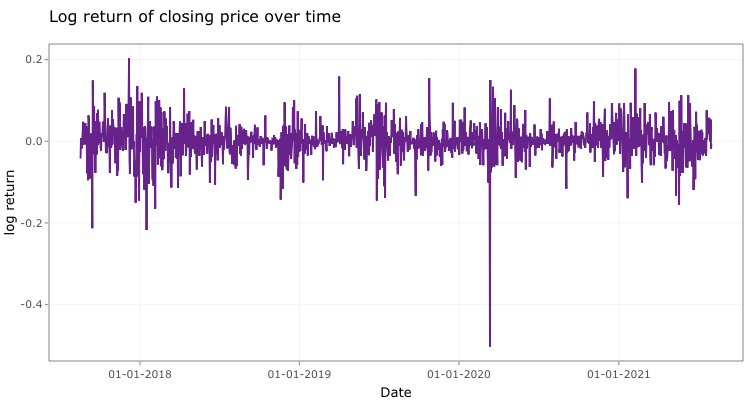
\includegraphics[width=\linewidth]{Extremal Modelling/logreturn_17_21.png}
    \caption{The daily log return of Bitcoin process from August 2017 to August 2021. Notice the very large drop in March of 2020.}
    \label{fig:logreturn_17_21}
\end{figure}

In light of this, it is not unnatural to ask the corresponding statistical question in the context of extremes. In Figure \ref{fig:hist_logreturn_17_21}, we can see that the distribution of log returns for our data set admits very heavy tails. Admittedly, one is aware of the very large anomaly which greatly negatively skews the data in a noticeable fashion. However, in spite of this, using a common statistical rule for eliminating outliers based upon the quartiles of a distribution, we find, as in Figure \ref{fig:distplots_sans_outliers}, the data still exhibits this skewed behaviour. This sparks interest in using extreme value theory to aid our understanding of it. \begin{figure}
    \centering
    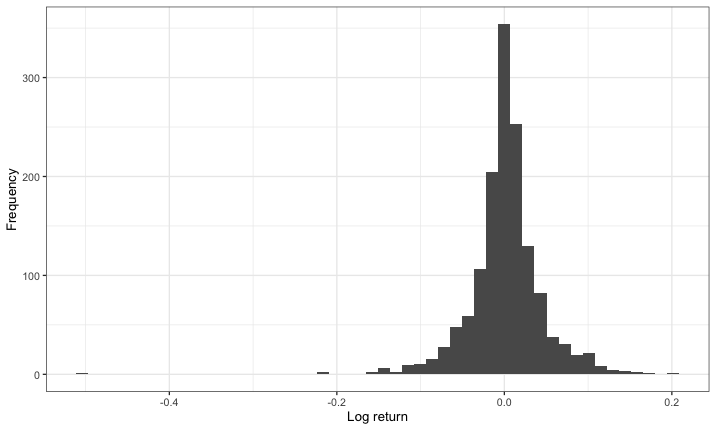
\includegraphics[width=\linewidth]{Extremal Modelling/hist_logreturn_17_21.png}
    \caption{Distribution of log returns using data from August 2017 to August 2021. The distribution shows some quite heavy tails.}
    \label{fig:hist_logreturn_17_21}
\end{figure}

\begin{figure}
    \centering
    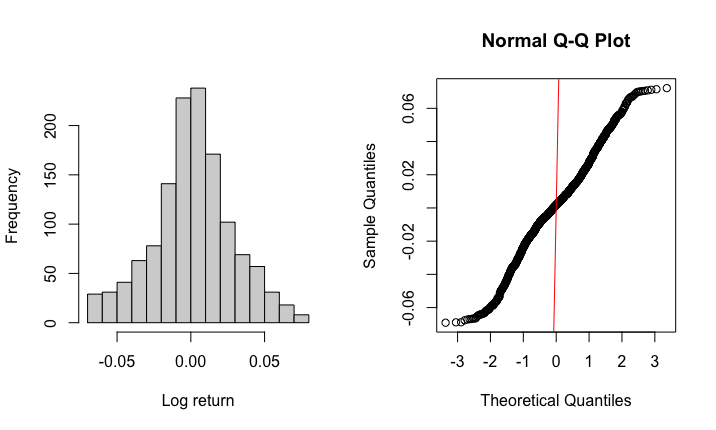
\includegraphics[width=\linewidth]{Extremal Modelling/distplots_sans_outliers.png}
    \caption{Distribution of log returns having eliminated outliers and a QQ plot of the data against a standard normal random variable. Clearly the data is still heavily tailed.}
    \label{fig:distplots_sans_outliers}
\end{figure}








\end{spacing}
\end{document}
